% Chapter 1
% !TeX spellcheck = en_US 
\chapter{Neural networks} % Main chapter title

\label{Chapter3} % For referencing the chapter elsewhere, use \ref{Chapter1} 
\setcounter{chapter}{3}
%\setcounter{section}{0}
In the \nameref{Chapter1} chapter, we breifly talked about a neural network which can be used 
to recognize hand-written digits. The neural network takes an image of a hand-written digit as 
an input and predicts a number which corresponds to the digit as an output. In this chapter, 
we will delve deeper into the architecture of neural networks and try to answer the following questions:
\begin{enumerate}
    \item What is the motivation behind using neural networks ?
    \item What is the idea behind the structure (neurons, input layer, hidden layers, output layer) 
    of neural networks ?
    \item Why do we need an activation function and a loss function ?
    \item How to train a neural networks ?
    \item What are learning algorithms ?
    \item Why certain neural networks can approximate any continuous function defined on a compact set ?
\end{enumerate}
Recognition of handwritten digits is a classic problem for introducing the topic of neural networks. Therefore 
we will use this problem as an example to introduce various concepts related to neural networks.
% \begin{figure}[htbp]
%     \centering
%     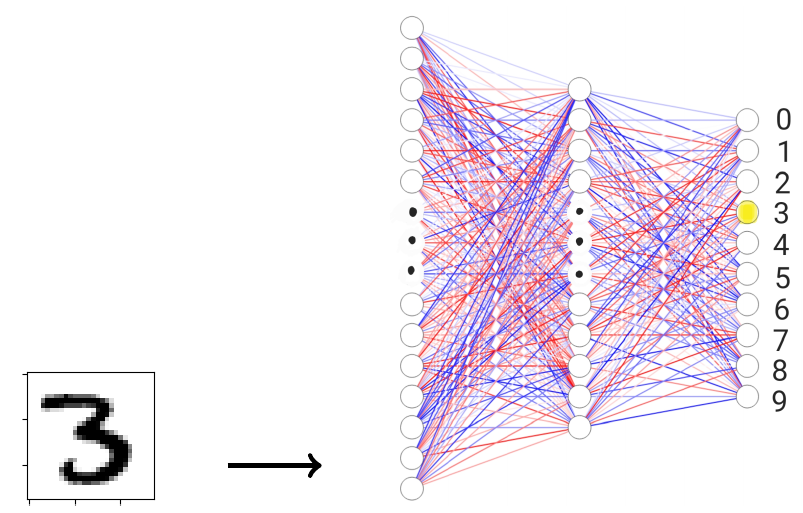
\includegraphics[width=0.8\textwidth]{Figures/ff_net.png}
%     \caption{A feed-forward neural network which can recognize hand-written digits.}
%     \label{fig:ffnet}
% \end{figure}   
%%%%%%%%%%%%%%%% Handwritten digit recog %%%%%%%%%
\section{Handwritten digit recognition}
Most people can easily recognize the handwritten digits shown in figure \ref{fig:my_digits}. Even if these digits were written 
in a different manner (for example refer figure \ref{fig:my_threes} ), one would still be able to recognize them. 
\begin{figure}[htbp]
    \centering
    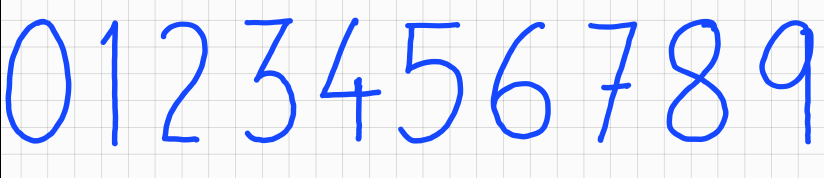
\includegraphics[width=.6\textwidth]{Figures/digits.png}
    \caption{One of the ways of writing digits from $1$ to $9$.}
    \label{fig:my_digits}
\end{figure} 
\begin{figure}[htbp]
    \centering
    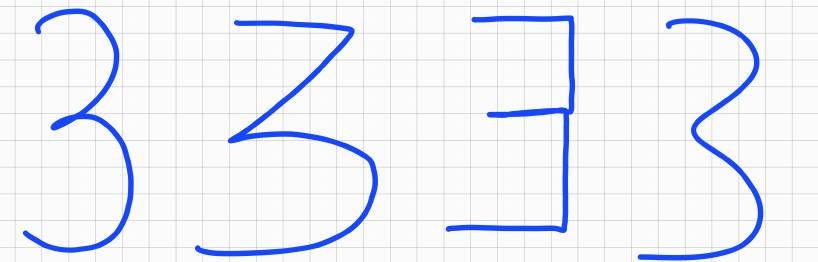
\includegraphics[width=.3\textwidth]{Figures/three_digit.png}
    \caption{Different ways of writing the digit $3$.}
    \label{fig:my_threes}
\end{figure} This is due to the fact that our visual cortex has evolved over millions of years and therefore is magnificently 
adapted to understand the visual world. The problem of recognizing hand-written digits is so trivial 
for our brains that we don't have to put an effort to recognize digits. But this task will immediately 
start to look complicated when one tries to write a computer program which can recognize hand-wriiten 
digits. 
Let us try to write a program for this task. We can start by coverting the digits into a pixel 
image ($28 \times 28$ for example) and assign each a value from $0$ to $1$ based upon the level of darkness
of each pixel (figure \ref{fig:pix7}). This can serve as an input to our program. 
\begin{figure}[htbp]
    \centering
    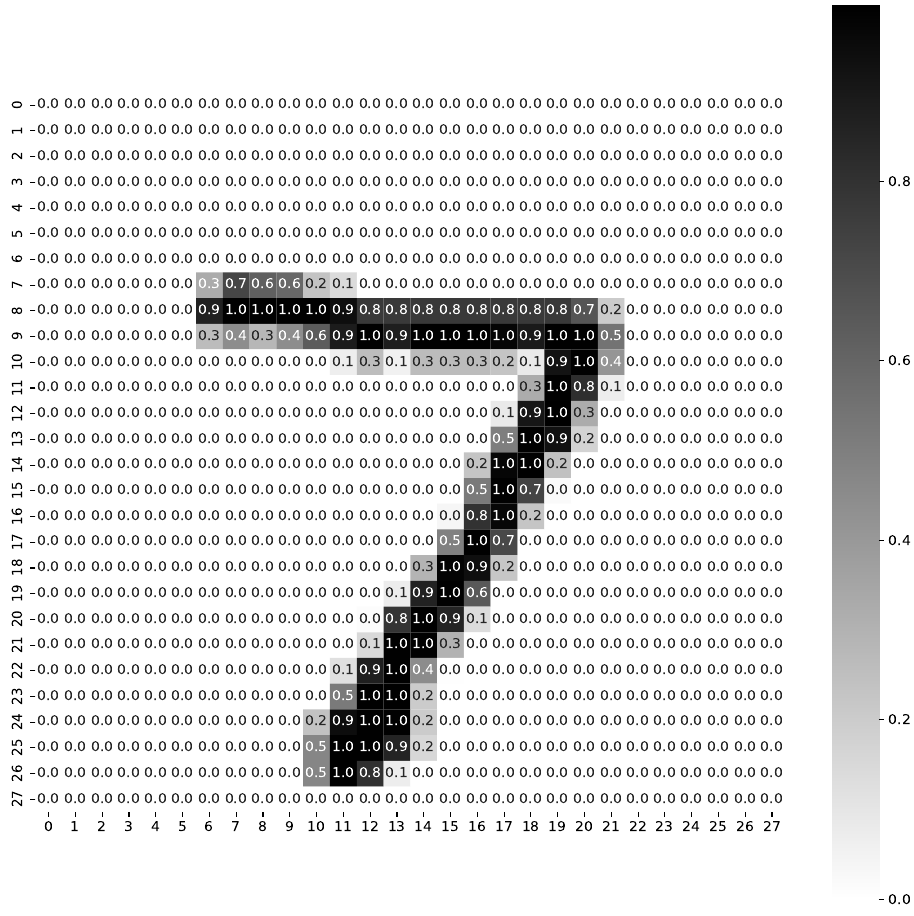
\includegraphics[width=.35\textwidth]{Figures/pixel_image_7.png}
    \caption{A $28 \times 28$ pixel image of digit $7$. Each pixel is assigned a value from $0$ to $1$.}
    \label{fig:pix7}
\end{figure} 
We can identify distinct features of each digit and write code which looks for these features in the input image. 
Our program will therefore contain a lot of \emph{if} statements and \emph{for} loops to identify such features 
but more importantly will contain thousands of line of code to handle exceptions which arise from the fact that 
each digit can be written in a slightly different manner. It turns out it is very difficult to express algorithmically 
the intuitions we have to recognize digits. Soon we will realize the complexity of this task. What if we could write a 
program (for such fuzzy and difficult to-reason-about problems) that mimics the structure of our brain ?  
% \begin{figure}
%     \centering
%     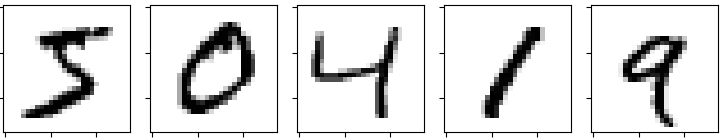
\includegraphics[width=.6\textwidth]{Figures/mnist_digits.png}
%     \caption{A sample of hand-written digits taken from MNIST dataset.}
%     \label{fig:mnist}
% \end{figure} 
% \begin{figure}
%     \centering
%     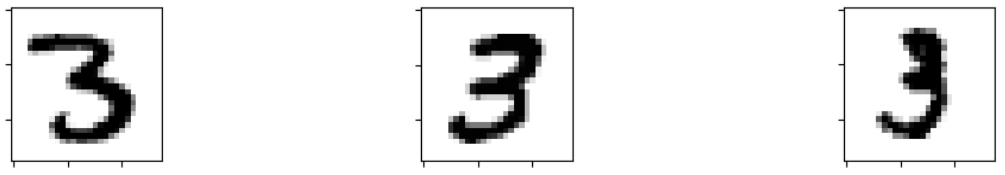
\includegraphics[width=.7\textwidth]{Figures/mnist_3s.png}
%     \caption{A sample of hand-written digit $3$ taken from MNIST dataset.}
%     \label{fig:mnist_3s}
% \end{figure} 
%%%%%%%%%%%%%%%% Intro to NN %%%%%%%%%%%%%
\section{Introduction to neural networks}
Neural networks tackles this problem in a different way. The construction of neural network
is inspired by the structure of our brain. 
\begin{figure}[htbp]
    \centering
    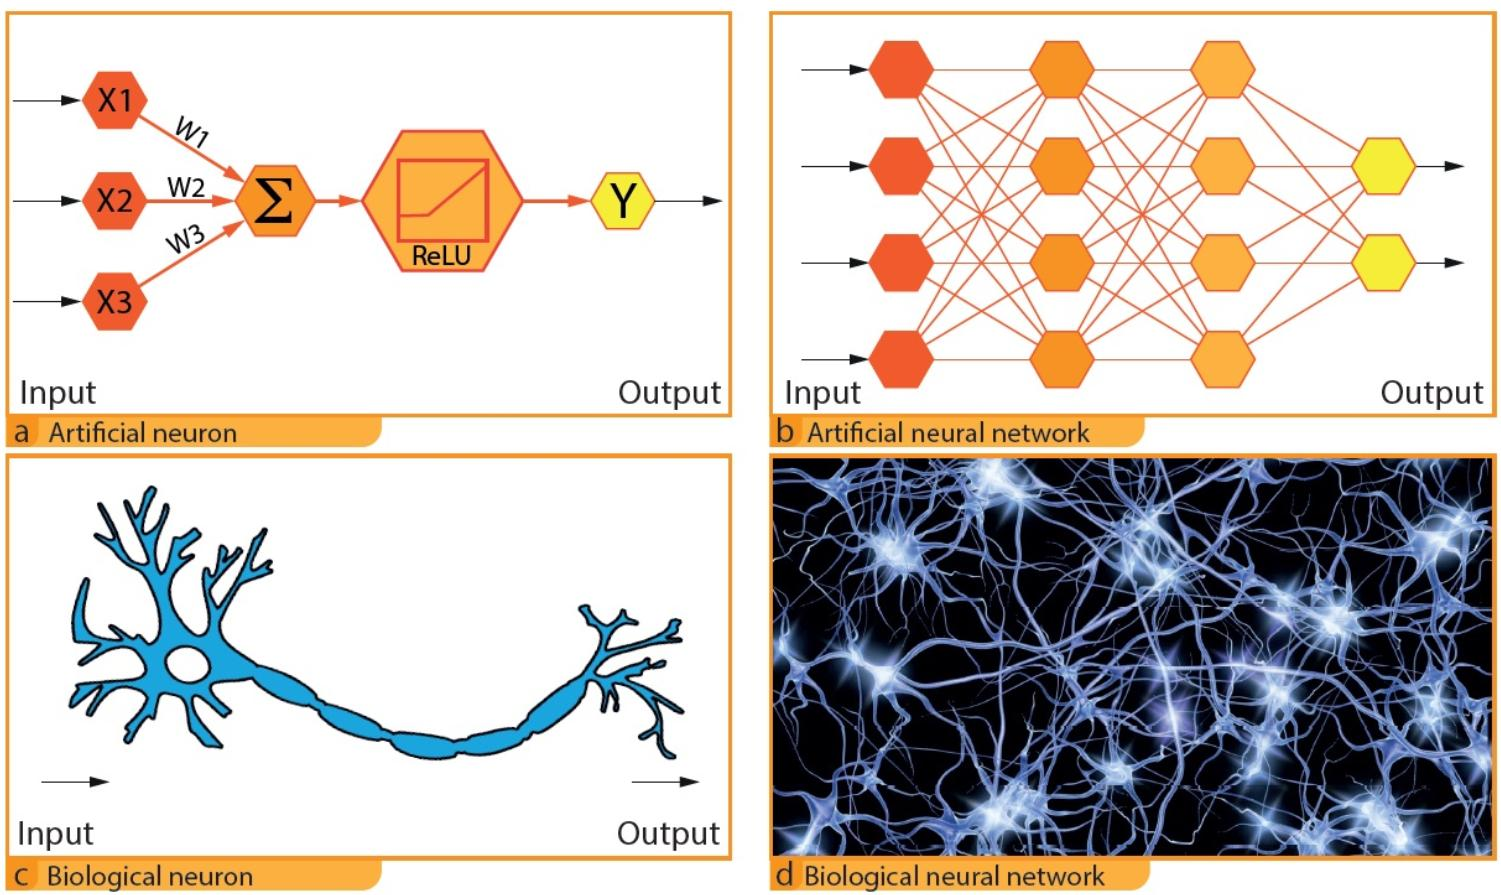
\includegraphics[width=.5\textwidth]{Figures/artificial_vs_normal_neurons.png}
    \caption{Similarity between the structure of artificial and biological neuron.}
    \label{fig:bio_neu}
\end{figure} 
The idea is to take a large number of handwritten digits together with labels and develop a system 
which can learn from these examples just like we learn. We leave it to the system to automatically infer rules 
from these examples and classify hand-written digits. 
\begin{figure}[htbp]
    \centering
    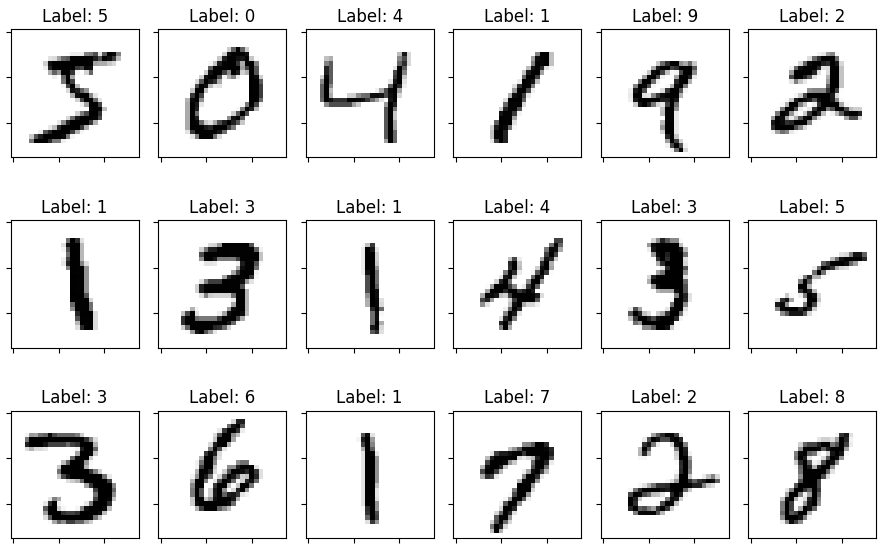
\includegraphics[width=.5\textwidth]{Figures/training_examples_mnist.png}
    \caption{Some training examples from MNIST dataset.}
    \label{fig:train_MNIST}
\end{figure} 

A neural network takes an input and given an output. Figure \ref{fig:ff_net} shows a pictorial representation of
a neural network which can be used to classify handwritten digits. It has layers (input, hidden, output) which consist of 
artificial neurons. The neurons are connected. Each neuron stores a value (for example from $0$ to $1$ in 
our case of handwritten digit recognition). 
\begin{figure}[htbp]
    \centering
    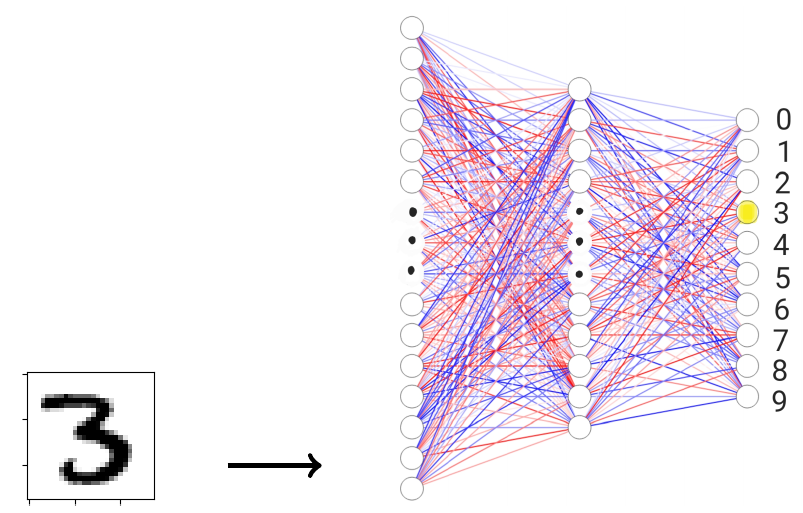
\includegraphics[width=.8\textwidth]{Figures/ff_net.png}
    \caption{A neural network to classify handwritten digits}
    \label{fig:ff_net}
\end{figure} 
A neuron takes multiple inputs (say $a_1, a_2,....,a_n$) and gives the output $\sigma(\sum_{i =1}^n a_i w_i + b)$ where $\sigma$ is
called an activation function. The inputs are multiplied by weights, $w_i$ and added to bias, $b$ before passing through the activation funciton.
The choice of activation function depends on the type of problem one is trying to solve. For example, for hand-written digit recognition one could use sigmoid/logistic function
as an activation function. 
\begin{figure}[htbp]
    \centering
    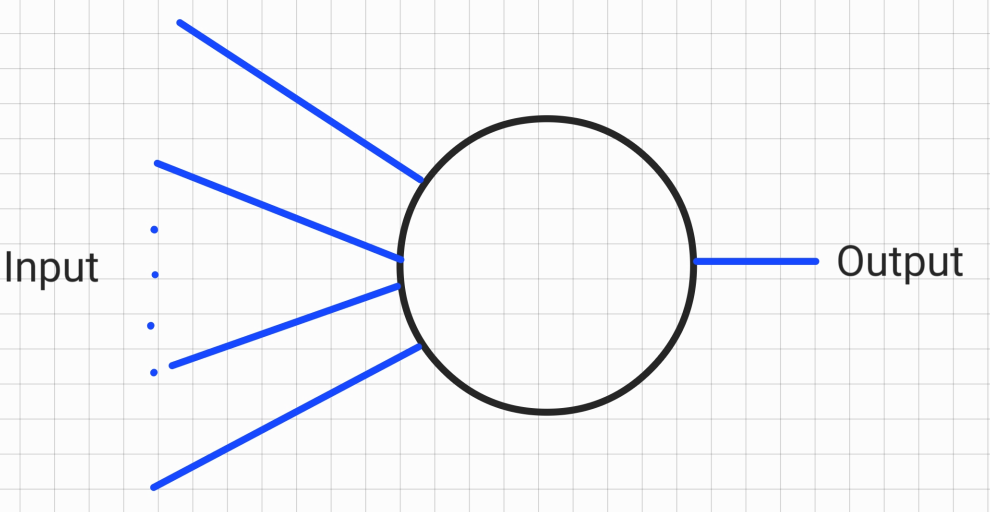
\includegraphics[width=.4\textwidth]{Figures/neuron.png}
    \caption{Pictorial representation of an artificial neuron. Elaborate}
    \label{fig:neuron}
\end{figure} 
\begin{figure}[htbp]
    \centering
    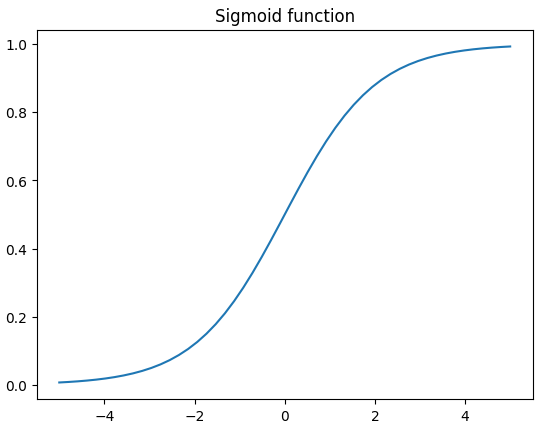
\includegraphics[width=.4\textwidth]{Figures/sigmoid.png}
    \caption{A sigmoid/logistic activation function, $\sigma (z) = \frac{1}{1+ e^{-z}}$}
    \label{fig:sig}
\end{figure} 

Mathematically speaking, a neural network is simply a function that takes an input which passes through
its layers (made up of neurons which are mathematical functions) and results in an output. The neural 
network shown in figure \ref{fig:ff_net} has $784$ neurons in the input layer (containing data from a $28 \times 28$ pixel image), $15$
neurons in the hidden layer and $10$ neurons in the output layer. Each neuron in the output layer corresponds to a digit from $0$ to $9$; if
the input image is of digit $3$, only the fourth neuron in the outplayer will light up (output is close to $1$) while the rest will remain dormant (outputs are close to $0$).
Such neural networks are called feed-forward neural networks. When we look at the architecture of a neural network, many questions can 
come to our mind, for example, 
\begin{enumerate}
    \item Why the network has this structure (i.e. layers with neurons) ?
    \item What is the purpose of using an activation function ?
    \item How does a neural network able to recognize hand-written digits ?
\end{enumerate} 
It is not clear why this appraoch of using neural networks even works. Even if we assume that this approach works, another question arises,
which is, how do we get the weights, $w_i$ and biases $b_i$ of the network ? The answer to this question
comes from a key ability of neural networks which is \emph{learning}.
%%%%%%%%%%%%%%%% Learning from data %%%%%%%%%%%
\subsection{Learning from data}
Learning is the process of obtaining suitable weights and biases such that a neural network can perform
the desired task. There are several steps involved in learning. First step is to assign random values to 
weights and biases of the network and show the network some training examples. In the case of handwritten digit recognition
we use MNIST dataset. Since the network is initialized with random weights and biases it will wrongly classify handwritten digits. 
\begin{figure}[htbp]
    \centering
    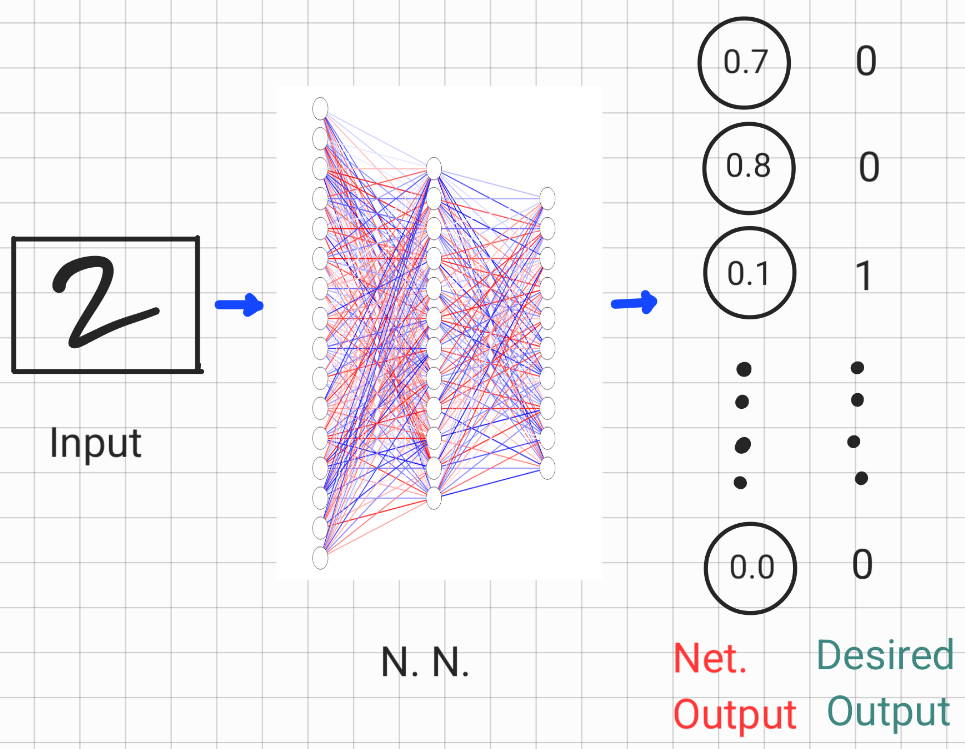
\includegraphics[width=.4\textwidth]{Figures/rand_inp.png}
    \caption{Results from a randomaly initialized neural network and how it compares to the desired output for a training example}
    \label{fig:randinp}
\end{figure} 
Next step is to tell the network to update its weights and biases in order to reduce the classfication error. This is done by introducing a 
cost/loss function which can quantify the classification error. We use a quadratic loss function, 
$$C(w,b) = \frac{1}{N} \sum_x {\|y(x) - a\|}^2$$
where $N$ denotes the number of training examples, $y(x)$ is the desired output corresponding to training example $x$, and 
$a$ is the neural network output. Our aim is to find $w,b$ such that the loss is minimum. The problem of learning from training data thus translates into
solving an optimization problem. But this process raises another set of questions,
\begin{enumerate}
    \item Which optimization algorithm to choose for minimizing the cost function?
    \item How to define a suitable loss function ?
    \item Does a global minimum exists for a chosed loss function ?
\end{enumerate}
The answer these questions and the questions that we raised earlier we will have to first understand the origins of neural networks.
%%%%%%%%%%%%%% Origins of NN %%%%%%%%%%%%%%
\subsection{Origins of neural networks}
The artificial neurons we introduced earlier are called sigmoid neurons. In order to understand 
why sigmoid neurons are defined the way they are, we need to first understand another artificial 
neuron called perceptron. Perceptrons were developed in the $1950$s and $1960$s. Unlike sigmoid neurons 
whose inputs, $x_i \in \mathbb{R}$, a perceptrons can take only binary inputs and produce a binary output.
The mathematical model of a perceptron is,
\begin{equation*}
    \text{output} = 
     \begin{cases}
       0 &\quad \text{if} \ \ \sum_i w_i x_i \leq \ \text{threshold} \\
       1 &\quad  \text{if} \ \ \sum_i w_i x_i > \ \text{threshold} 
     \end{cases}
\end{equation*}
where $x_i$ are the inputs and $w_i$ are the weights. The output is $1$ if $\sum_i w_i x_i$ exceeds a threshold 
value otherwise the output is $0$. Perceptrons can be used as a device to make simple decisions by weighing up evidence. 
The following example illustrates how perceptrons can be used to make a decision.
\begin{boxedexample}
    Suppose a rock band is coming to perform in your city. You like rock music, and are trying to 
    decide whether or not to go to this event. You can make the decision by weighing up three factors:
   \begin{enumerate}
    \item Is the event nearby ?
    \item Are your friends accompanying you ?
    \item Is the weather good ?
   \end{enumerate}
   We can assign binary variables $x_1, x_2$ and $x_3$ to these three factors. For example, if the event is nearby we would
   have $x_1 =1$ but if it is far away we would have $x_1 = 0$. Similarly, if your friends are accompanying you, $x_2 =1$ otherwise $x_2 =0$.
   If the weather is good, $x_1 =0$ and if the weather is bad, $x_3 =0$. Now suppose, you absolutely love rock music and it doesn't really 
   matter to you if your friends can accompany you or if the event is nearby but you really loathe bad weather and you won't go if the
   weather is bad. You can use perceptrons to model this kind of decision-making. One way is to choose, $w_3 = 6$ for the weather and
   $w_1 =2, w_2 =2$ for other conditions. The larger value of $w_3$ in comparison to $w_1$ and $w_2$ suggests that weather matters to you a lot. 
   Finally, suppose you choose a thresold value of $5$ for the perceptron. With these choices, the perceptron mimics the desired 
   decision-making model, outputting $1$ whenever the weather is good, and $0$ whenever the weather is bad. By choosing different values for 
   weights and the thresold, we can get different models of decision making. 
\end{boxedexample}
It is obvious that the perceptron isn't a complete model of human descision-making. But it is plausible that if we use more layers in the network
with more number of perceptrons, the network could make more complex descisions:
\begin{figure}[htbp]
    \centering
    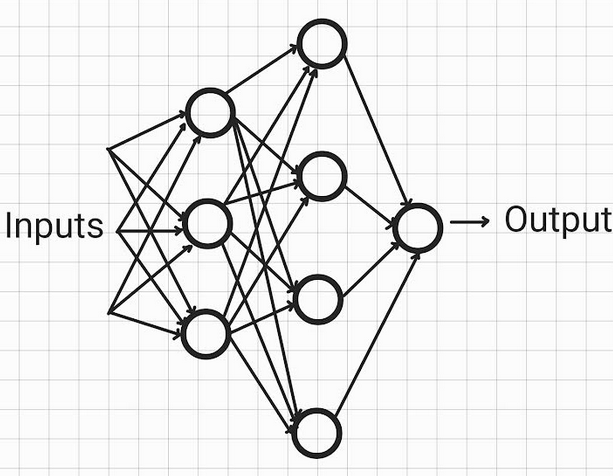
\includegraphics[width=.4\textwidth]{Figures/perceptron_network.png}
    \caption{A network built out of perceptrons.}
    \label{fig:percep_net}
\end{figure} 
We can write the mathematical model of a perceptron in a way familiar to us, 
\begin{equation*}
    \text{output} = 
     \begin{cases}
       0 &\quad \text{if} \ \ \sum_i w_i x_i + b \leq 0 \\
       1 &\quad  \text{if} \ \ \sum_i w_i x_i + b > 0 
     \end{cases}
\end{equation*}
where perceptron's bias, $b \equiv -$threshold. We have seen that a network of perceptrons can be used as 
a method for weighing evidence to make decisions. We can also use perceptrons to compute the elementary logical functions such as
AND, OR, and NAND. The NAND gates are universal for computation, and therefore it follows that perceptrons are also universal for
computation. This property of perceptrons tells us that networks of perceptrons can be as powerful as any other computing device. These 
properties of perceptrons might make them an attractive option for solving decision-making problems but the property that we 
are really looking for in the network is the ability to tune its weights and biases in response to external stimuli (for example training data).
We want our network to learn from data. In order to devise learning algorithms for a network, we would like that if we make 
a small change in some weight (or bias) in the network, the output changes only by a small amount. Schematically, here's is what we want:
\begin{figure}[htbp]
    \centering
    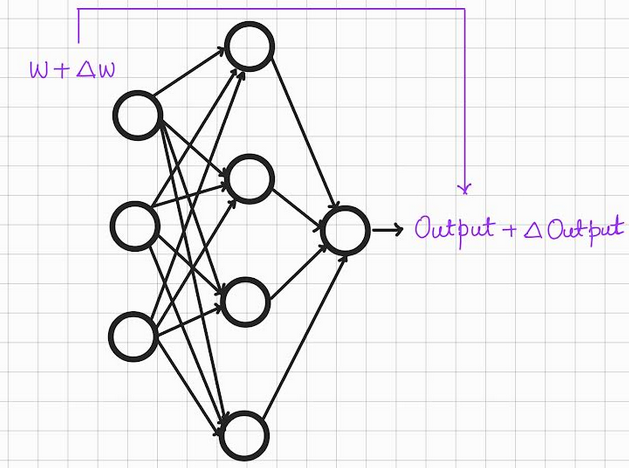
\includegraphics[width=.4\textwidth]{Figures/precepnet2.png}
\end{figure}
 
Unfortunately, a network of perceptrons doesn't have this capability. This is the reason why we use sigmoid neurons. Unlike perceptrons, the sigmoid 
neurons can take input values between $0$ and $1$. The activation function used in sigmoid neurons can be described as, 
$$\sigma(z) = \frac{1}{1 + e^{-z}}.$$
The smoothness of $\sigma$ ensures that a small change in the input causes a small change in the output. 

Figure \ref{fig:deepNN} shows an architecture of a typical (feed-forward) neural network. It consists of an input layer, multiple hidden layers and an output layer. The choice of
the number of neurons in the input and output layers is governed by the problem one is trying to solve. For example, in the case of 
hand-wriiten digit recognition, if the input image consists of data from $28 \times 28 = 784$ pixels, the input layer will have $784$ neurons. We want to classify the 
images into digits from $0$ to $9$ and therefore the output layer will have $10$ neurons. The design (number of layers and number of neurons) of hidden layers
is based on heuristics. Let us now look at a neural network (in detail) which can classify handwritten digits. 
\begin{figure}[htbp]
    \centering
    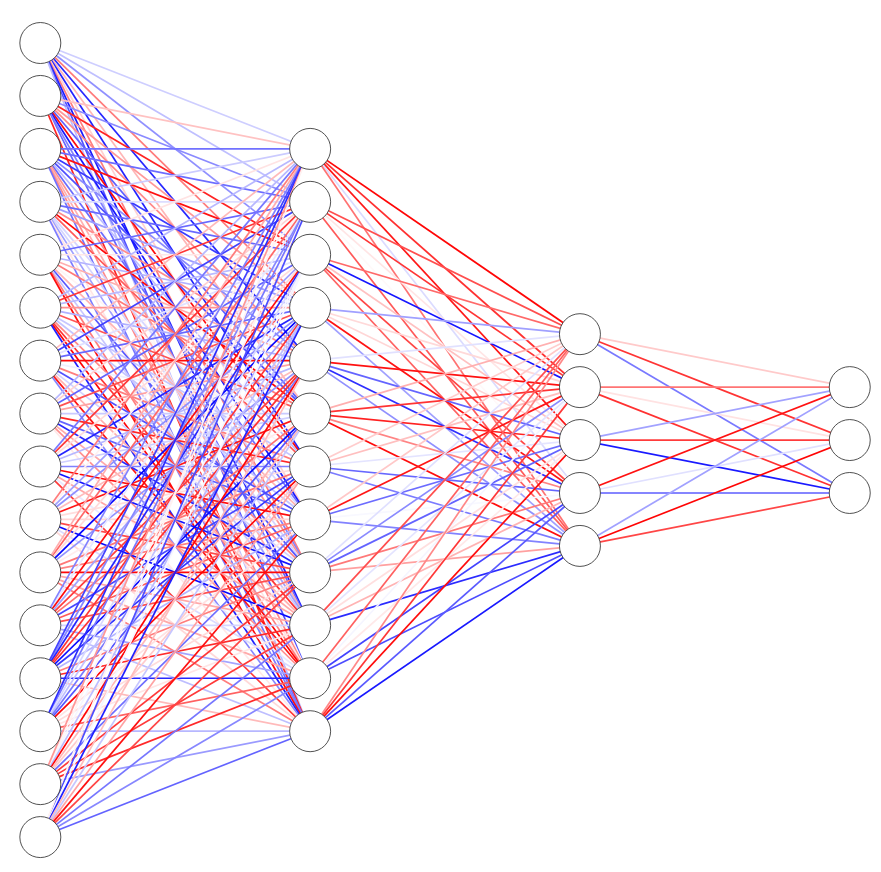
\includegraphics[width=.4\textwidth]{Figures/DeepNN.png}
    \caption{A feedforward neural network with an input layer $\in \mathbb{R}^{16}$, two hidden layers and an output layer $\in \mathbb{R}^2$.}
    \label{fig:deepNN}
\end{figure}
%%%%%%%%%%%% network to classify HD %%%%%%%%%%%%
\subsection{A network to classify handwritten digits}
We use a network consisting of an input layer $\in \mathbb{R}^{784}$, one hidden layer and an output layer $\in \mathbb{R}^{10}$ to classify handwritten
digits (see figure \ref{fig:NN_HD}). Let us try to understand how this neural network works. 
\begin{figure}[htbp]
    \centering
    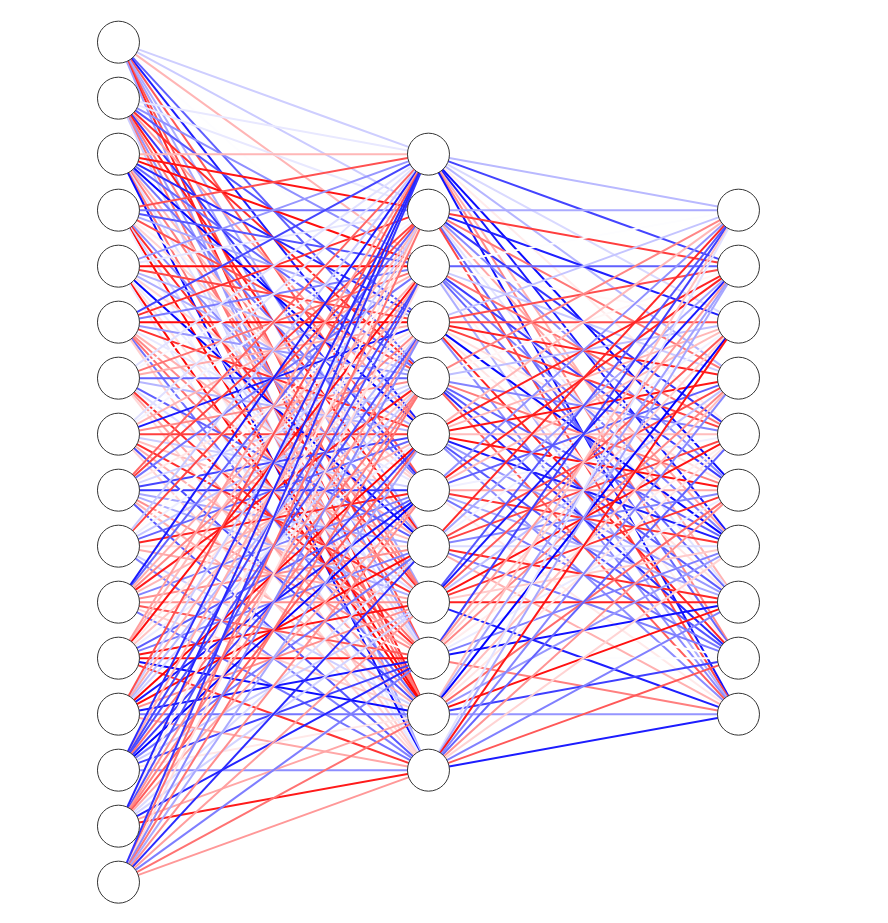
\includegraphics[width=.4\textwidth]{Figures/NN_2.png}
    \caption{A neural network which can classify handwritten digits.}
    \label{fig:NN_HD}
\end{figure} 
The main feature of this network is its ability to learn from data. We use MNIST data set which consists of scanned images of handwritten digits written by $250$ people. The MNIST data
comes in two parts; a training data set containing $60000$ imgaes and a test data set containing $10000$ images. The images are in grescale and have size of $28 \times 28$ pixels.
The MNIST data, along with hand-written digits, also provide correct labels corresponding to the digits. 
\begin{figure}[htbp]
    \centering
    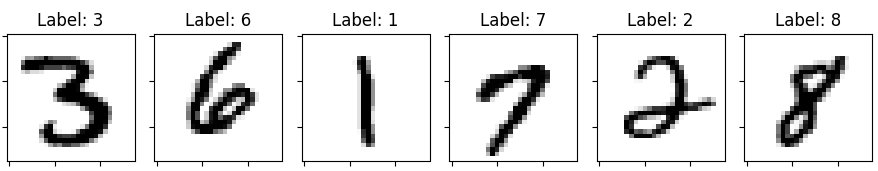
\includegraphics[width=.4\textwidth]{Figures/mnist_data_sample.png}
    \caption{A sample of training data from MNIST data set.}
    \label{fig:mnist_data}
\end{figure} 
The input $x$ to the network is a $28 \times 28 = 784$ dimensional vector and the output $a$ is a $10$ dimensional vector. In order to quantify, the 
accuracy of this network's prediction, we define a cost/loss function,
$$C(w,b) = \frac{1}{N} \sum_x {\|y(x) - a\|}^2$$
where $N$ denotes the number of training examples, $y(x)$ is the desired output (a $10$ dimensional vector) corresponding to a training example $x$, and 
$a$ is the neural network output. The idea is to find weights and biases which minimizes the difference between the desired output (labels) and the network prediction and we want this to happen for all training examples. For example, 
if an input $x$ is an image of digit $6$, we want our network's output $a$ to be as close as possible to $y(x) = (0,0,0,0,0,0,1,0,0,0)^T$. The problem of 
minimizing the loss function is an optimization problem. In the context of neural networks, the most popular methods which are used to minimize the loss function are 
inspired from the gradient descent method. 

Let us consider a simple example to understand the gradient descent method. Suppose we want to minimize a function $C(\mathbf{v})$ of two variables $v_1$ and $v_2$ (see figure \ref{fig:cost_f}).
\begin{figure}[htbp]
    \centering
    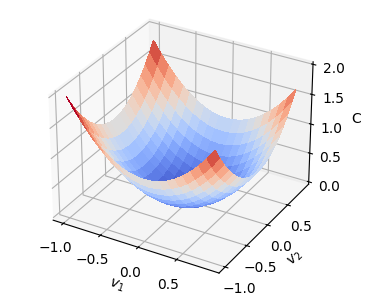
\includegraphics[width=.4\textwidth]{Figures/cost_func.png}
    \caption{A function $C$ of two variables $v_1$ and $v_2$.}
    \label{fig:cost_f}
\end{figure} 
We can use calculus to calculate the gradients of $C(\mathbf{v})$ with resprect two $v_1, v_2$ and use them to find places where $C$ is minimum. This method could work well when 
$C$ is a function of few variables but soon will turn into a nightmare when we increase the number of variables. Typically, the cost function of a neural network depends on a large number of
weights and biases; in fact the biggest neural networks consists of billions of weigths and biases. Therefore, one has to come up with cost effective 
methods of finding the minima of cost functions. Grandient descent is one such method. It is an interative method, where one starts 
with an initial guess for variables and update them over multiple iterations in such a 
way that the cost function reduces with each iteration. Consider the case of cost function $C(\mathbf{v}$). For small changes $\Delta v_1$ and  $\Delta v_2$ in variables $v_1$ and 
$v_2$ respectively, we can write the change in cost function $\Delta C$ as
\begin{equation}
    \label{eq:del_C}
    \Delta C \approx \frac{\partial C}{\partial v_1}\Delta v_1 + \frac{\partial C}{\partial v_2} \Delta v_2 = \nabla C \cdot \Delta \mathbf{v}
\end{equation}
The aim is to find suitable change $\Delta \mathbf{v}$ which leads to reduction in $C$ i.e. $\Delta C < 0$. One such choice is $\Delta \mathbf{v} = -\eta \nabla C$ provided $\eta > 0$,
$$\Delta C \approx \nabla C \cdot \eta \nabla C = \eta \|\nabla C\|^2 < 0 $$
To conclude, in the gradient descent method we start with an initial guess $\mathbf{v}$ and update it by following
 $$\mathbf{v} \rightarrow \mathbf{v}' = \mathbf{v} - \eta \nabla l$$
untill we reach the minimum of $C(\mathbf{v})$. In the context of neural networks, a gradient descent update might look like this, 
\begin{equation}
    \begin{aligned}
        w_j \rightarrow w_j' = w_j - \eta \frac{\partial C}{\partial w_j}\\
        b_k \rightarrow b_k' = b_k - \eta \frac{\partial C}{\partial b_k}.
    \end{aligned}
\end{equation}
Note that the parameter $\eta$ should be sufficiently small in order to justify the assumption in equation \eqref{eq:del_C}. 
We call this parameter the \emph{learning rate}. The use of gradient descent method might seem as a
good alternative to using analytical methods but there are still a number of challenges in applying this method. Notice that the cost function has the form
$C = \frac{1}{N} \sum_x C_x$, that is, it's an average overs costs $C_x = \|y(x) - a\|^2$ for individual training examples. In order to make an update of gradient
descent, we need to compute the gradients $\nabla C_x$ separately for each training input and then average them, $\nabla C = \frac{1}{N} \sum_x \nabla C_x$. This update can take 
extremely long time to make when the number of training inputs are very large and thus making the \emph{learning} very slow. 

We can overcome the issue of slow \emph{learning} by using a variant of gradient descent method known as \emph{stochastic gradient method}. The idea is to estimate the gradient
$\nabla C$ by computing $\nabla C_x$ for a small sample of training examples and use it to make updates in weights and biases. The following steps are involved in using the stochastic gradient descent method,
\begin{enumerate}
    \item Shuffle the training inputs and divide into batches of size $m$. Each batch (we call them mini-batchs) consits of training examples say, $X_1, X_2, .....X_m$.
    \item Calculate gradients for one mini-batch: $$\frac{1}{m} \sum_{i=1}^{m} \nabla C_{X_i} \approx \frac{1}{N} \sum_x \nabla C_x = \nabla C$$
    \item Make an update in the weights and biases: 
    $$w_j \rightarrow w_j' = w_j - \frac{\eta}{m} \sum_i \frac{\partial C_{X_i}}{\partial w_j}$$
    $$b_k \rightarrow b_k' = b_k - \frac{\eta}{m} \sum_i \frac{\partial C_{X_i}}{\partial b_k}$$
    \item Pick another mini-batch from the shuffled data and repeat steps $2$ and $3$ until all training inputs are exhausted. The end of this step is referred to as an \emph{epoch} of training.
    \item Repeat steps $1$ to $5$ until the network is sufficiently trained.
\end{enumerate}
The use of stochastic gradient significantly increases the speed at which a network is trained. We may be making less accurate updates (hence the name \emph{stochastic}) in the weights and biases in comparison to 
standard gradient descent method but nevertheless the updates are faster and over multiple iterations the cost (on an average) does go down.   
%%%%%%%%%%% UAT %%%%%%%%%%%%%%%%%%%%%
\section{The universal approximation theorem}
Neural networks are mathematical functions. We use training data to look for suitable weights and biases
such that the neural network can map/obtain the underlying function from which the data is drawn. But, how can one
believe that a neural network have the capability of finding the underlying function. What is so special about the
neural network structure that after training it is able to give us great results on unseen data/ test data ? The answer to these
questions lies in the universal approximation theorem (UAT) proposed by George Cybenko in $1989$. 
George Cybenko gave a rigorous proof that feed-forward neural networks can approximate any continuous function defined on a compact set. To understand the 
proof of this theorem, one should be familiar with some concepts from measure theory and functional analysis. 
Let us first briefly go through those mathematical preliminaries.
\begin{itemize}
    \item Consier an $n$-dimensional unit cube, $I_n = [0,1]^n$. In the universal approximation theorem, the continuous
    functions that a neural network aims to approximate are defined on compacts sets, $I_n$ i.e. the domain of continuous
    functions is $I_n$. 
    \item Let $C(I_n)$ denote the space of continuous functions on $I_n$.
    For any function $f \in C(I_n), f : [0,1]^n \rightarrow \mathbb{R}$, one can define a suitable norm, 
    $\|f\| = \text{sup}_{x \in I_n} |f(x)|$ known as uniform/supremum norm. We can associate a dual space to $C(I_n)$ 
    defined as $C(I_n)* = \{L : C(I_n) \rightarrow \mathbb{R}\}$ where $L$ is a linear operator.
    \item UAT is defined for feed-forward neural networks having an input layer (with multiple neurons), one hidden layer and
    an output layer with only one neuron (see figure \ref{fig:ffnn_UAT}). Therefore, the functions generated by the neural network can be described as
    $$G(x) = \sum_{j=1}^{N} \alpha_j \sigma (w_j\cdot x + b_j), \quad w_j \in \mathbb{R}^n, \alpha_j, b_j \in \mathbb{R}, x \in I_n$$
    where $N$ is the number of neurons in the hidden layer. We can note that bias is not added to output from the hidden
    layer. Also the output is not passed to an activation function. We denote the set of functions of the form $G(x)$
    by $\mathcal{N}$. In the problem of hand-written digit recognition, we assumed that the activation function, $\sigma$ is logistic/sigmoid. 
    However, UAT was proved for a general class of activation functions. The actvation functions are assumed to be continuous and 
    discriminatory. 
\end{itemize} 
\begin{figure}[htbp]
    \centering
    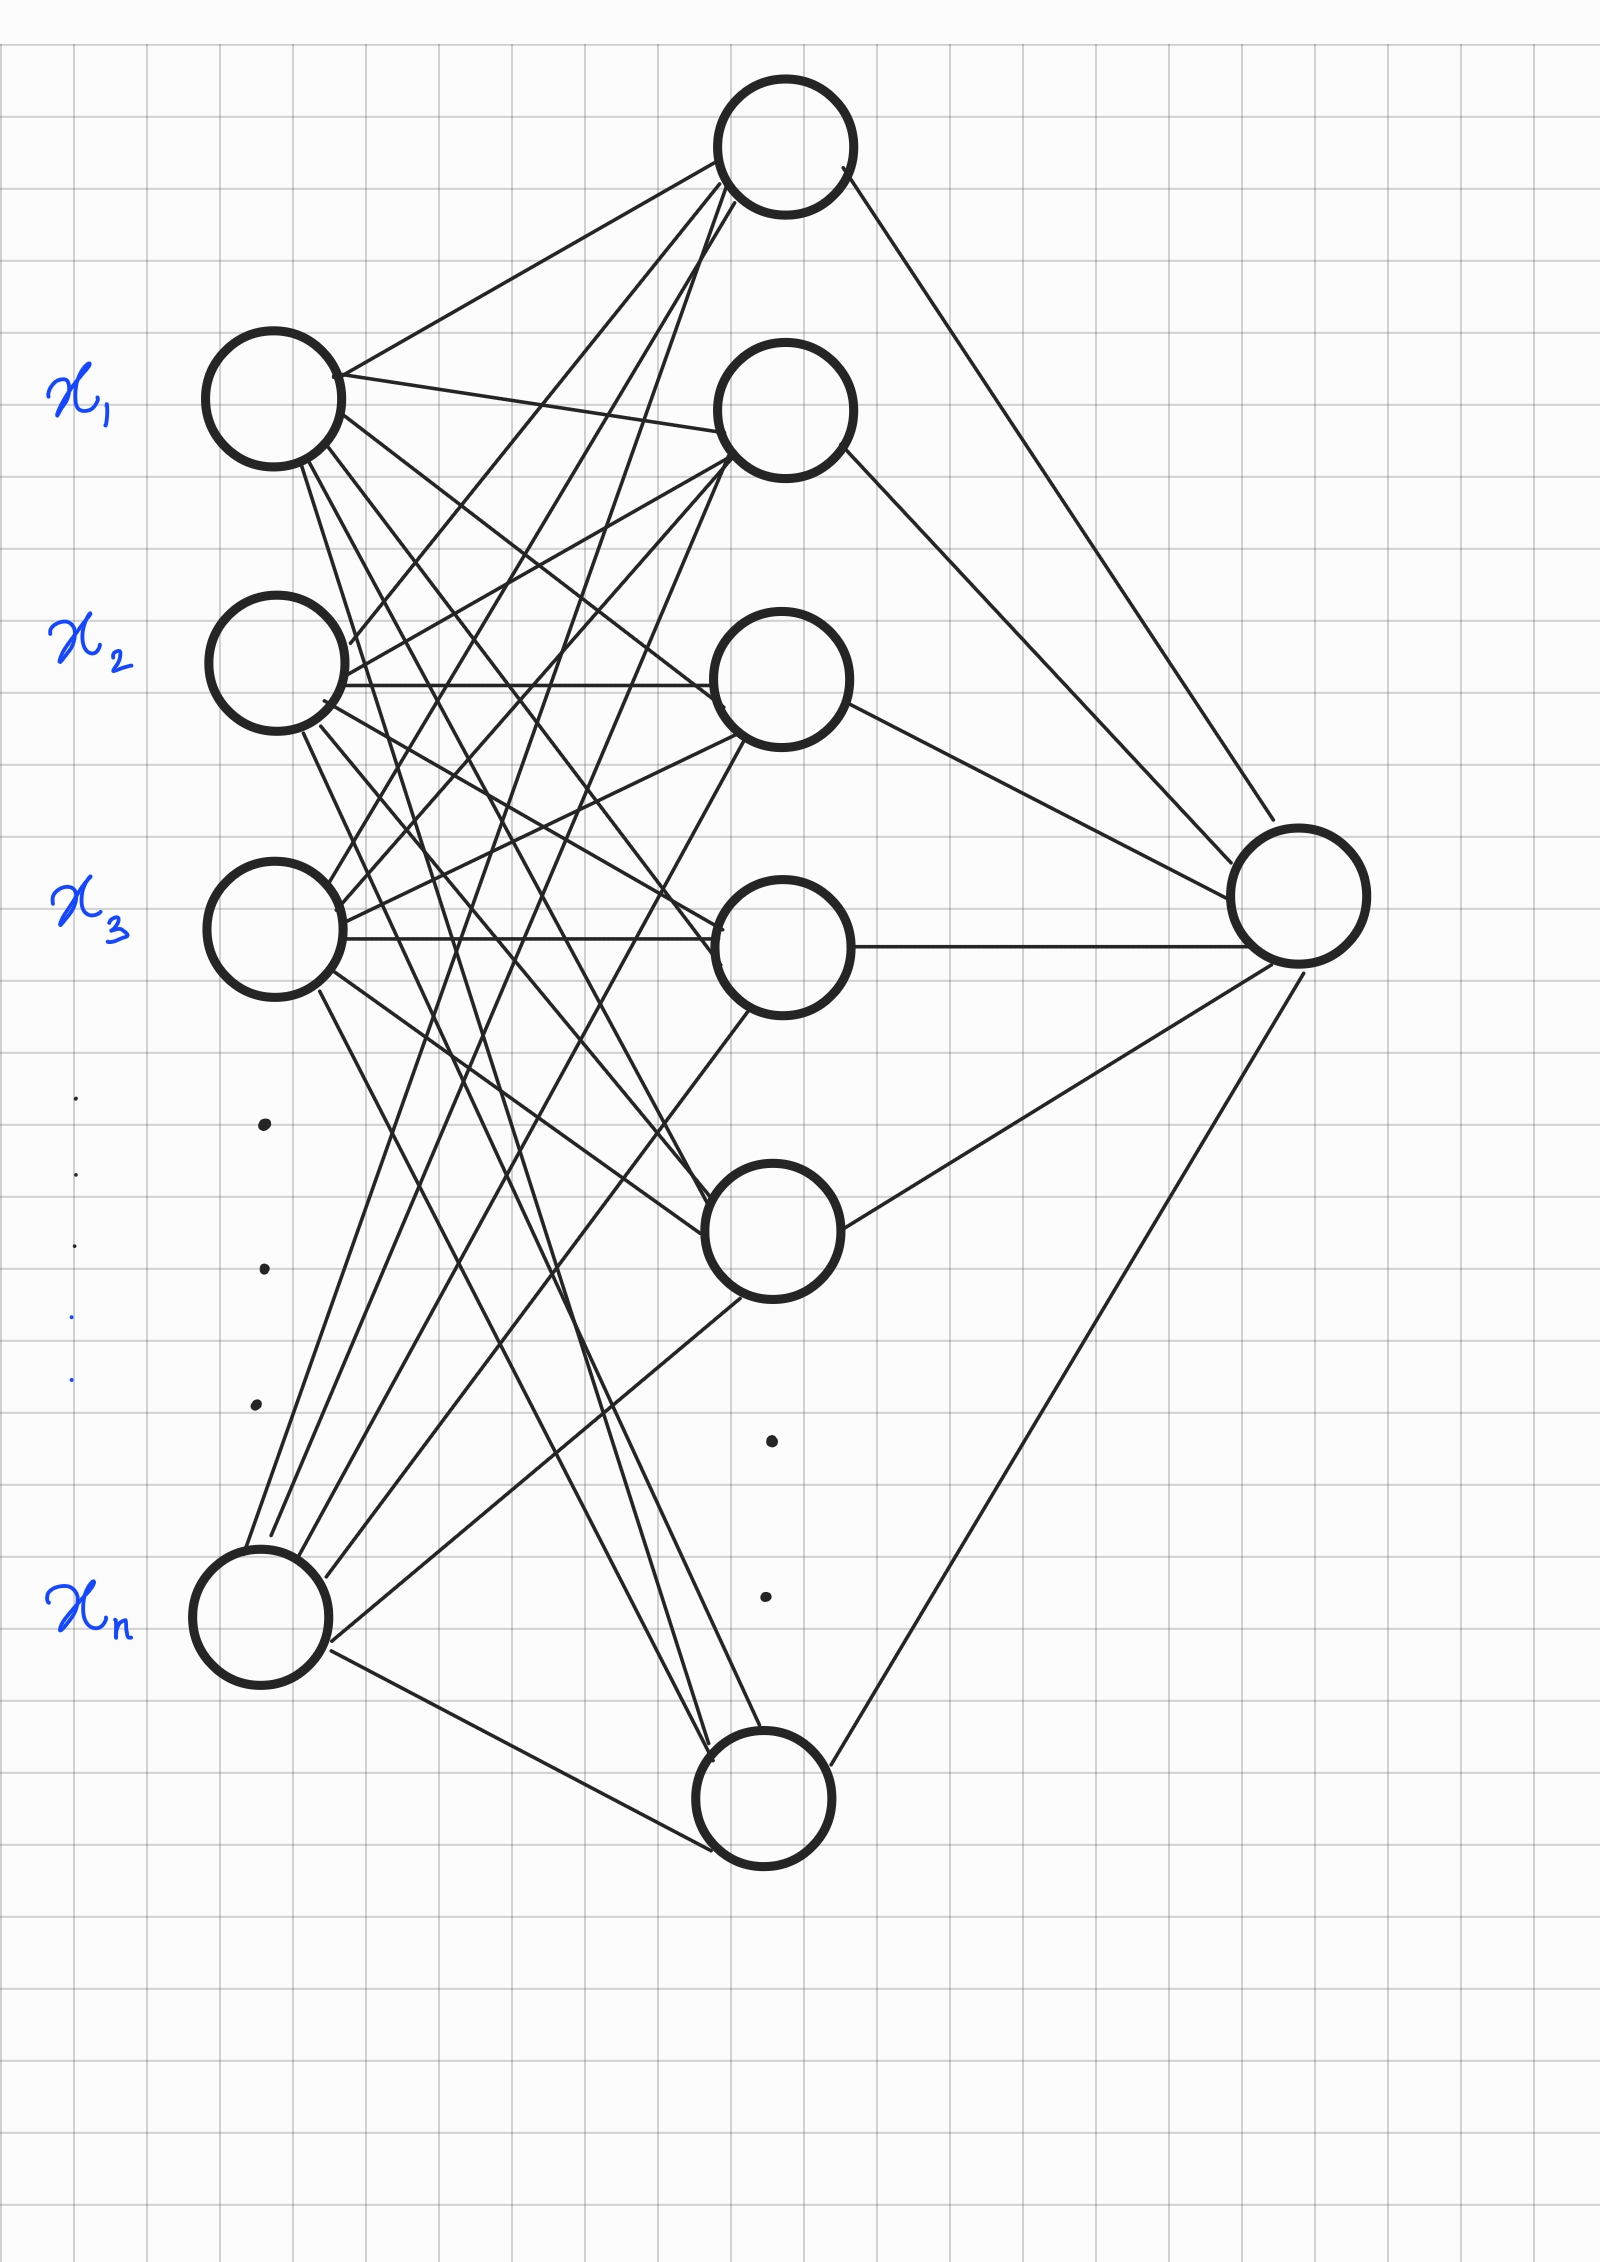
\includegraphics[width=.4\textwidth]{Figures/ffnn_UAT.jpg}
    \caption{A feed-forward neural network with an input layer (having multiple neurons), one hidden layer and an output layer (having only one neuron).}
    \label{fig:ffnn_UAT}
\end{figure}
\begin{definition}[Discriminatory function]
    We say that $\sigma$ is discriminatory if for a measure $\mu \in M(I_n)$ (where $M(I_n)$ is the space 
of finite, signed regular Borel measures on $I_n$) 
$$\int_{I_n} \sigma (\mathbf{w}\cdot\mathbf{x} + b) \ d\mu(\mathbf{x}) = 0$$
for all $\mathbf{w} \in \mathbb{R}^n$ and $b\in \mathbb{R}$ implies that $\mu = 0$.
\end{definition}
\begin{thm}[Universal approximation theorem]
    \label{thm:UAT}
    Let $\sigma$ be any continuous discriminatory function. Then the set $\mathcal{N}$ of functions of the form 
    $$G(x) = \sum_{j=1}^{N} \alpha_j \sigma (w_j\cdot x + b_j), \quad w_j \in \mathbb{R}^n, \alpha_j, b_j \in \mathbb{R}, x \in I_n$$
    are dense in $C(I_n)$. In other words, given any function $f \in C(I_n)$ and $\epsilon > 0$, there exists
    a $G(x) \in \mathcal{N}$ such that 
    $$\| G(x) - f(x)\| < \epsilon \ \text{for all} \ x \in I_n$$
\end{thm}
Before going into the proof of UAT, we will familiarize ourselfves with some key ideas from measure theory.
\begin{itemize}
    \item Our aim to measure subsets of $I_n = [0,1]^n$. A collection $\sum$ of subsets of $I_n$ is called a 
    $\sigma$-algebra if 
    \begin{enumerate}
        \item $I_n \in \sum$
        \item If $A \in \sum$, then $A^c = I_n\backslash A \in \sum$
        \item If $A_1, A_2, .....$ is a countable collection of subsets of $\sum$ then $\bigcup^\infty A_i \in \sum$.
    \end{enumerate}
    \item Borel $\sigma$-algebra on $I_n$ is the smallest $\sigma$-algebra  containing all open sets in $I_n$. Sets in Borel $\sigma$-algebra 
    are called Borel sets.
    \item A finite signed Borel measure $\mu$ on $I_n$ is a real valued  function, $\mu : \sum \rightarrow \mathbb{R}$  (where
    $\sum$ is a Borel $\sigma$-algebra defined on $I_n$) such that 
    \begin{enumerate}
        \item $\mu (\phi) = 0$
        \item $\mu (\bigcup_{i=1}^{\infty} A_i) = \sum_{i=1}^{\infty} \mu(A_i), A_i \ \text{are disjoint sets}$
        \item $\mu(A_i) < \infty$
    \end{enumerate}
    \item A Borel measure is regular if 
    \begin{align*}
        &\mu(A) = \text{sup} \{\mu(K) | K \subseteq A, K \ \text{is compact}\} \\
        &\mu(A) = \text{inf} \{\mu(U) | A \subseteq U, U \ \text{is open}\}
    \end{align*}
    In other words, what regular means is every measurable set can be approximated from above by open measurabel 
    sets and from below by compact measurable sets. 
    \item We define $M(I_n)$ as the set of all finite signed regular Borel measures on $I_n$.
\end{itemize}
The proof of UAT also uses ideas from Hahn-Banach theorem and Riesz representation theorem. These theorems 
have various equivalent versions. We now define the versions which we will refer to later. 
\begin{thm}[Riesz representation theorem]
    \label{thm:RR}
    If $K \subset \mathbb{R}^d$ is a compact set, then every linear functional $L$ defined on
    $C(K)$ can represented by a unique regular signed Borel measure $\mu \in M(K)$ in the sense that,
    $$L(f) = \int_K f \ d\mu$$
    where $f: K \rightarrow \mathbb{R}$.
\end{thm}
\begin{thm}[Hahn-Banach theorem]
    \label{thm:HB}
    Let $M$ be a linear subspace of a normed linear space $X$, and $f_0 \in X$. Then $f_0$ is 
    in the closure $\overline{M}$ of $M$ if and only if there is no bounded linear functional 
    $L$ on $X$ such that $L(f) = 0 $ for all $f\in M$ but $L(f_0) \neq 0$.
\end{thm}
We now give the proof of universal approximation theorem \ref{thm:UAT}.
\begin{proof}
   $C(I_n)$ is a vector space equipped with a supremum norm and hence is a normed vector space. It is
   clear that the set formed by functions of the form $G(x)$ is a subset of $C(I_n)$ i.e. $\mathcal{N} \subset C(I_n)$.
   We claim that $\mathcal{N}$ is also a linear subspace of $C(I_n)$. This is true due to the fact that if 
   we take two functions $G_1(x), G_2(x) \in \mathcal{N}$, we can always find a function $G_3(x) \in \mathcal{N}$ such that 
   $G_3(x) = \alpha G_1(x) + \beta G_2(x)$ for all $\alpha, \beta \in \mathbb{R}$. Our next claim is that the closure of 
   $\mathcal{N}$ is all of $C(I_n)$ i.e. $\mathcal{N}$ is dense in $C(I_n)$. We prove this by contradiction. 

   Assume that the closure of $\mathcal{N}$, $\overline{\mathcal{N}}$ is not all of $C(I_n)$ i.e. 
   $\overline{\mathcal{N}} \neq 0$. It can be proved (refer any standard functional analysis book) that $\overline{\mathcal{N}}$
   is a closed proper subspace of $C(I_n)$.  By Hahn Banach theorem \ref{thm:HB}, there exists a bounded 
   linear functional on $C(I_n)$, let's call it $L$, with the property that $L \neq 0$ but $L(\overline{\mathcal{N}}) = L(\mathcal{N}) = 0$.
   By following Riesz representation theorem \ref{thm:RR}, we can write this linear operator, $L$ as 
   $$L(h) = \int_{I_n} h(x) \ d\mu(x)$$
   for some $\mu \in M(I_n) \forall h \in C(I_n)$. Since this operator returns $0$ for all elements of $\mathcal{N}$,
   we must have for all $w \in \mathbb{R}^n, b \in \mathbb{R}$ 
   $$\int_{I_n} \sigma (w \cdot x + b) \ d\mu(x) = 0.$$
   However, we assumed that $\sigma$ is a discriminatory functions therefore this condition implies that $\mu =0$. This contradicts our initial assumption that 
   $\overline{\mathcal{N}} \neq 0$ which led to $L \neq = 0 \equiv \mu \neq 0$ via Hahn Banach theorem. Hence, the subspace $\mathcal{N}$ must be dense in $C(I_n)$. 
\end{proof}
The universal approximation theorem gives us confidence that neural networks can indeed approximate any continuous function 
provided that the activation function is continuous and discriminatory. However, it is not clear how to build activation functions which are 
discriminatory.
\begin{definition}
    \label{def:sig}
    We say that $\sigma$ is sigmoidal if 
    \begin{equation*}
        \sigma(t) \rightarrow 
         \begin{cases}
           1 &\quad \text{as} \ \ t\rightarrow +\infty\\
           0 &\quad \text{as} \ \ t\rightarrow -\infty.
         \end{cases}
    \end{equation*}
\end{definition}
\begin{lemma}
    \label{lem:sig}
    Any continuous sigmoidal function is discriminatory.
\end{lemma}
\begin{proof}
    Refer Cybenko paper.
\end{proof}
The lemma \ref{lem:sig} gives us a way to build suitable activation functions. In fact, the sigmoid/logistic function we used as an activation function
in the neural network for solving hand-written recognition problem satisfies the conditions of definition \ref{def:sig} and is therefore, discriminatory. Although 
logistic function is monotonically increasing, no monotonicity is required by definition \ref{def:sig}.